\section{Diseño de la Plataforma}
\thispagestyle{plain}

\vspace{0.5cm}

\Large\scshape
\begin{center}
    \textrm{Diseño e implementación de los circuitos principales y auxiliares de la plataforma}
\end{center}
\normalfont
%\normalsize

\divider

Si bien con el análisis del anterior capítulo se pudo conseguir un panorama general del funcionamiento de la plataforma, se presentan otras complejidades a la hora de plasmarlo en un sistema real: se requieren múltiples circuitos auxiliares además de los bloques principales (por ejemplo circuitos de adquisición de señales); aparecen consideraciones de diseño que no existen en el plano teórico; entre otras cuestiones. Este capítulo está dedicado al diseño e implementación real de la plataforma completa en una placa de circuito impreso o PCB, teniendo en cuenta estas complicaciones.\\

En la siguiente figura se presenta un diagrama de la plataforma con un mayor detalle que el de la figura \ref{diag_plataforma}, dónde se pueden ver los distintos bloques auxiliares que va a ser necesario implementar.\\

\begin{figure}[h]
    \centering
    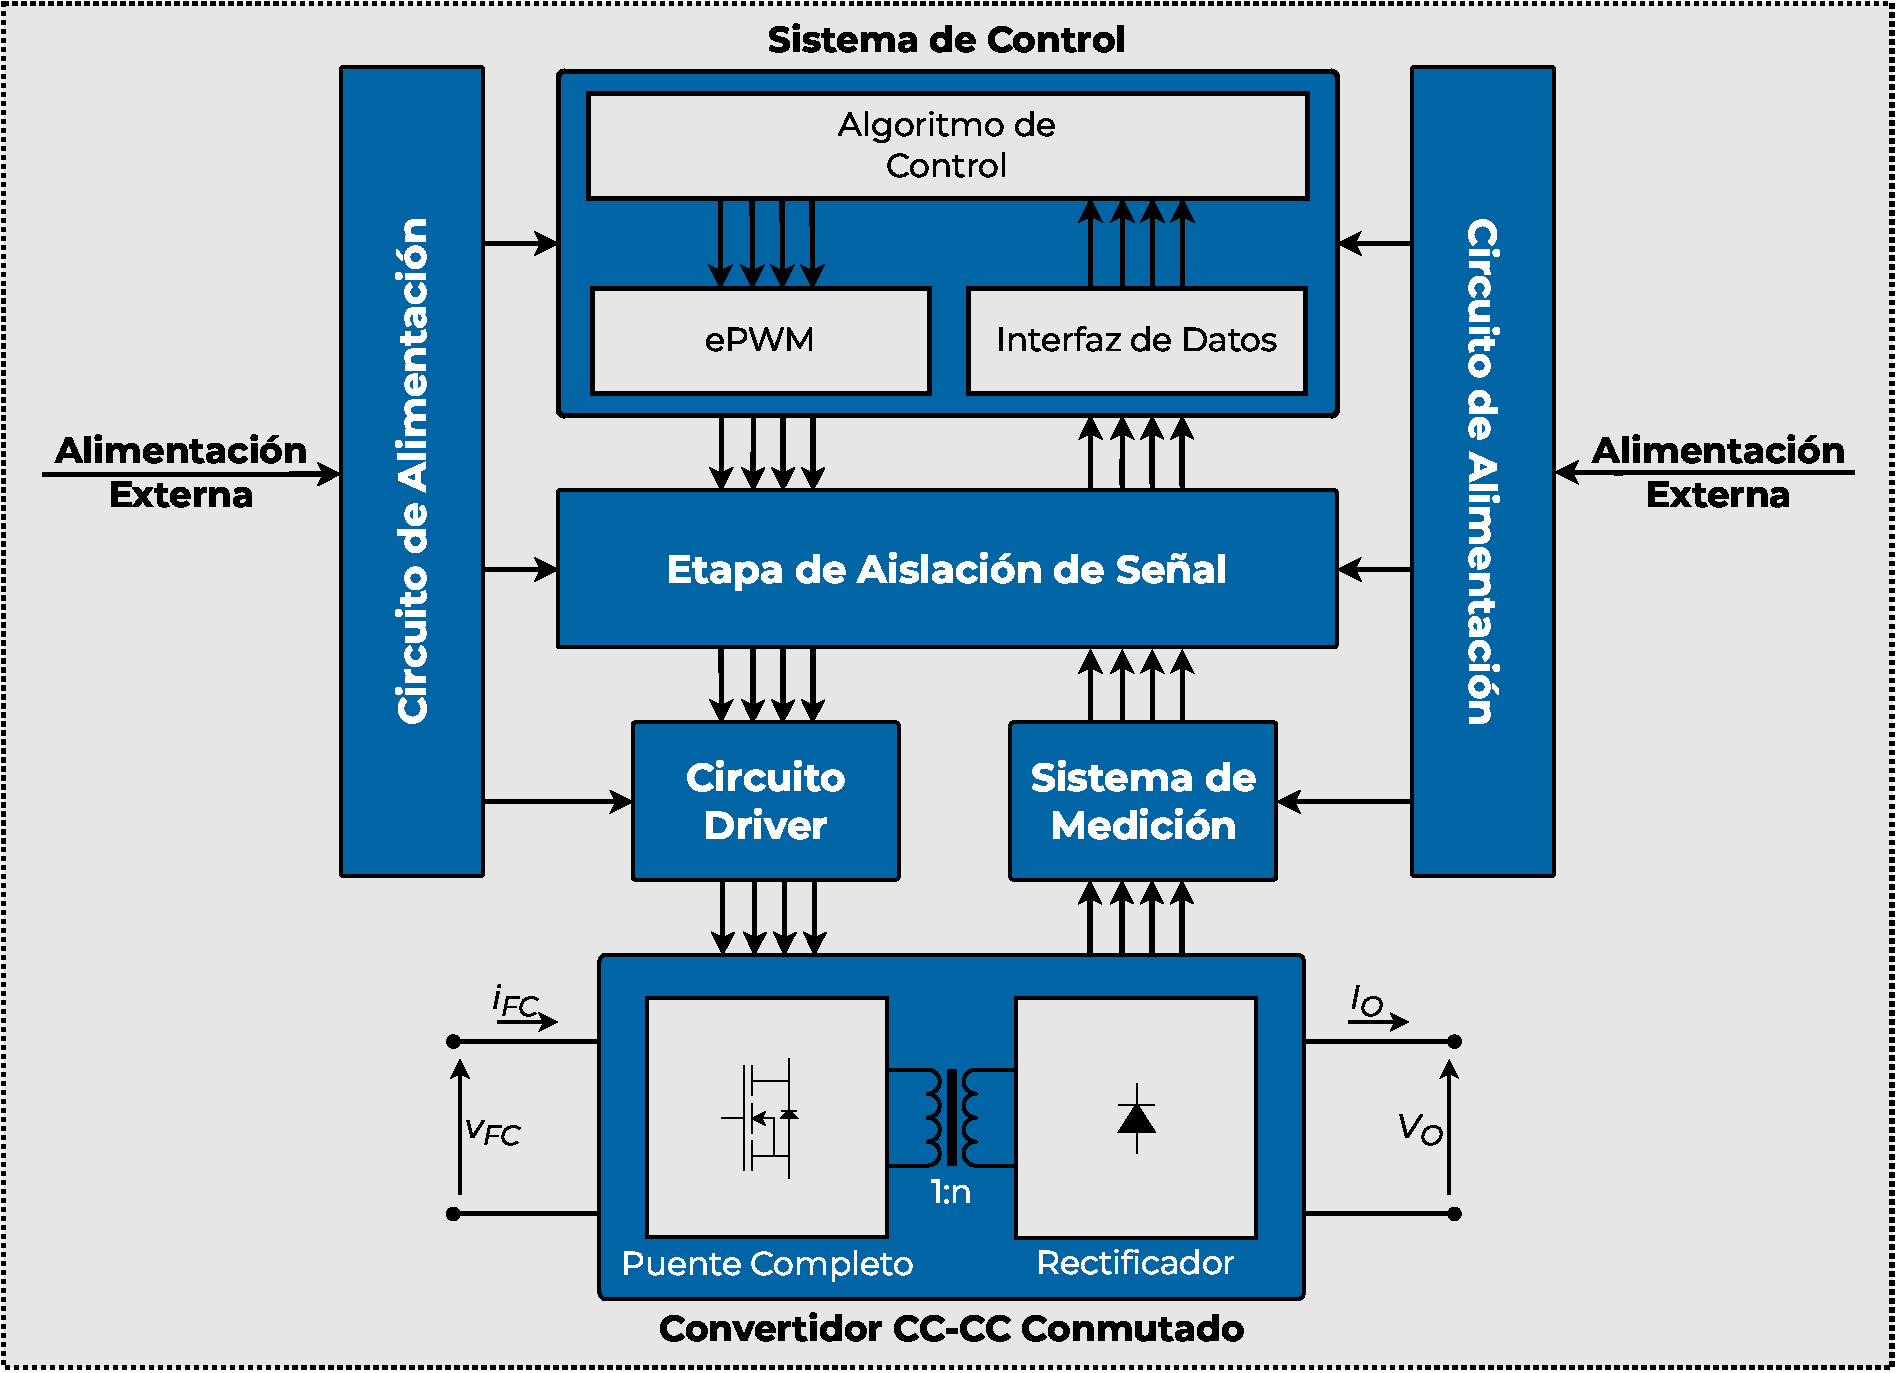
\includegraphics[scale=0.2]{Imagenes/Plataforma Detallada.pdf}
    \caption{Diagrama detallado de la plataforma de evaluación, incluyendo los distintos circuitos auxiliares (Placeholder).}
    \label{diag_detallado}
\end{figure}